\documentclass[12pt]{article}

\usepackage[utf8]{inputenc}
\usepackage{latexsym,amsfonts,amssymb,amsthm,amsmath}
\usepackage{tikz}
\usepackage{stanli}
\usetikzlibrary{calc,through}
\usepackage{multicol}
\usepackage{geometry} 
\usepackage{enumitem}

\definecolor{darkred}{rgb}{0.6,0,0}

\setlength{\parindent}{0in}
\setlength{\oddsidemargin}{-0.25in}
\setlength{\textwidth}{7in}
\setlength{\textheight}{9.3in}
\setlength{\topmargin}{-1in}
\setlength{\headheight}{18pt}

\newcommand\blfootnote[1]{%
  \begingroup
  \renewcommand\thefootnote{}\footnote{#1}%
  \addtocounter{footnote}{-1}%
  \endgroup
}

\title{ME473 Dynamic Finite Element Analysis Mini-Project}
\author{Stefano Burzio}
\date{}

\begin{document}
\noindent ME473 - Dynamic finite element analysis of structures\hfill EPFL\\
Stefano Burzio \hfill 2026\\
\vspace{0.3cm}

\hspace*{\fill}\textbf{\Large Mini-project 1}\hspace*{\fill}
\begin{center}
  \textbf{\Large Design of a 2d bridge}
\end{center}

\hrulefill
\vspace{0.3cm}
\newline
{Project organization:}
\vspace{0.2cm}
\newline
\begin{minipage}[t]{0.38\textwidth}
  \begin{itemize}[itemsep=0.005cm]
    \item Groups: 3 to 5 students
    \item 20\% of final grade
    \item Pdf report: maximum 10 pages
  \end{itemize}
\end{minipage}
\hfill
\begin{minipage}[t]{0.58\textwidth}
  \begin{itemize}[itemsep=0.005cm]
    \item Programming language: \texttt{MATLAB}
    \item Submission: November 13, 2026
    \item Total workload:  32h (approx. 8h per student)
  \end{itemize}
\end{minipage}
\vspace{0.3cm}

\hrulefill
\vspace{0.3cm}

You are tasked with designing and analyzing a 2d bridge using four fixed anchor points. The bridge must span a 20 meter gap and support a vertical point load applied at the center of the span.

\subsubsection*{Anchor points and load configuration}
The bridge connects the following four supports on a horizontal plane:
\begin{multicols}{2}
  \begin{itemize}
    \item Left outer: (–1, 0)
    \item Left inner: (0, 0)
    \item Right inner: (20, 0)
    \item Right outer: (21, 0)
  \end{itemize}
\end{multicols}
\vspace{0.3cm}
\begin{center}
  \begin{tikzpicture}
    % Nodes
    \def\c{0.7071}
    \def\s{0.7071}
    \coordinate (1) at (0,0);
    \coordinate (2) at (-1,0);
    \coordinate (3) at (10,0);
    \coordinate (4) at (11,0);
    \coordinate (5) at (5,2);
    %Supports 
    \point{a}{-1}{0};
    \point{b}{0}{0};
    \point{c}{10}{0};
    \point{d}{11}{0};
    \support{1}{a};
    \support{1}{b};
    \support{1}{c};
    \support{1}{d};
    % Members
    \draw[ultra thick] (1) -- (2);
    \draw[ultra thick] (3) -- (4);
    % Force at 1
    \draw[thin,dashed] (5,0) -- (5,2);
    \draw[thin,dashed] (0,0) -- (10,0);
    \draw[thick,latex-] (5,2.1)-- ++(0,1.2) node[midway,right] {50 kN};
    % Points
    \node[above=1pt,darkred] at (1) {1};
    \node[above=1pt,darkred] at (2) {2};
    \node[above=1pt,darkred] at (3) {3};
    \node[above=1pt,darkred] at (4) {4};
    \node[right=1pt,darkred] at (5) {5};
    % Dimensions
    \draw[|-|] (0,-1) -- node[below] {10 m} (5,-1);
    \draw[|-|] (5,-1) -- node[below] {10 m} (10,-1);
    \draw[|-|] (0,-1) -- node[below] {1 m} (-1,-1);
    \draw[|-|] (10,-1) -- node[below] {1 m} (11,-1);
    \draw[|-|] (4.5,0) -- node[left] {$a$} (4.5,2);
    % Pins
    \draw[thick,fill=white] (5) circle (3pt);
    \draw[thick,fill=white] (4) circle (3pt);
    \draw[thick,fill=white] (3) circle (3pt);
    \draw[thick,fill=white] (2) circle (3pt);
    \draw[thick,fill=white] (1) circle (3pt);
  \end{tikzpicture}
\end{center}

\subsubsection*{Truss design requirements}
The bridge must be modeled as both a planar truss and a planar frame. A vertical point load of 50 kN is applied at node 5, located at a defined height a, that can be chosen freely, and should represent a lower chord joints.

You are required both to perform both a static and a dynamic analysis for each of the three materials listed below, treating each case as a distinct full-bridge design. Compare the results obtains for each material and discuss the differences in terms of the modeling assumptions, planar truss vs planar frame.

\newpage
\begin{center}
  \begin{tabular}{l|c|c|c|c}
    {Material}          & {E (GPa)} & {Density (kg/m$^3$)} & {Cross-sectional area} & {Volume cap} \\
    \hline
    Structural steel    & 200       & 7850                 & 15–50 cm$^2$           & 1 m$^3$      \\
    Reinforced concrete & 30        & 2500                 & 300-600 cm$^2$         & 4 m$^3$      \\
    Engineered wood     & 12        & 600                  & 30–100 cm$^2$          & 1.7 m$^3$    \\
  \end{tabular}
\end{center}

\subsubsection*{Static analysis}
Each bridge design must strictly adhere to realistic structural behavior by ensuring static performance under load. This means the following two requirements must be satisfied:
\begin{enumerate}
  \item The entire structure must remain fully within the elastic range of the chosen material—no yielding or permanent deformation is allowed. Additionally, the displacement at any node must not exceed \textbf{40 mm}, in accordance with the L/500 criterion.
  \item Your designs should aim to optimize the total material volume. The total volume of the structure must not exceed the specified volume cap for each material.
\end{enumerate}

\subsubsection*{Dynamic analysis}
A separate modal analysis must be performed for each of the three trusses corresponding to the different materials. The following requirement must be satisfied:

\begin{enumerate}
  \item[3.] For each design, compute the first three natural frequencies and the corresponding mode shapes. The first natural frequency must \emph{not} fall within the range of \textbf{1.5 to 10 Hz}.
\end{enumerate}

\emph{Bonus 1}: To ensure dynamic stability and avoid resonance with common excitation sources, you should aim for a first natural frequency \textbf{above 50 Hz}, where feasible.

\emph{Bonus 2}: Reproduce one of your MATLAB models (either the planar truss or the 2D beam, for one selected material) in ANSYS. Perform static and modal analyses, then compare with your MATLAB results. Briefly explain any differences.


\subsubsection*{Deliverables}
\begin{enumerate}
  \item \texttt{MATLAB:}
        \begin{multicols}{2}
          \begin{itemize}
            \item Nodes and elements definitions
            \item Stiffness and mass matrices assembly
            \item Static and modal analysis
            \item Plots and visualizations
          \end{itemize}
        \end{multicols}


  \item \textbf{Report:}
        \begin{itemize}
          \item Truss layouts with labeled pins and bars,
          \item Summary of \texttt{MATLAB} results (displacements, stresses, frequencies and mode shapes),
          \item Discussion of your findings.
        \end{itemize}
\end{enumerate}

\end{document}